\newcommand{\question}[1]{\textit{\textcolor{Magenta}{#1}}}

\section{Teilversuch 2: Übergang von Fraunhofer- zu Fresnel-Beugung}
	\begin{itemize}
		\item \question{Wie lässt sich am Intensitätsverlauf die Anzahl der beteiligten Fresnel-Zonen bestimmen?}

			Man kann die Anzahl der beteiligten Fresnel-Zonen (im Zentrum) bestimmen, indem man die Anzahl der Peaks aufzählt. 

			In meinem Versuch war 11 Peaks beobachtet, also gibt es 5 Peaks und 5 Täler auf beiden Seiten des Zentralpeaks. Jedes Peak bezeichnet eine ungerade Anzahl von Fresnel-Zonen und jeder Tal eine gerade Anzahl. Wo die Intensität an beide Seite abnimmt, sind keine Fresnel-Zone mehr beteiligt. Mit dem Peak im Zentrum ergibt sich somit $11$ beteiligten Fresnel-Zonen. Aus Symmetriegründen kann man auch die Anzahl der Peaks direkt zählen, um die Anzahl der beteiligten Fresnel-Zonen zu bestimmen. 
		\item \question{Nehmen Sie parallele Beleuchtung des Spalts an und leiten Sie aus geometrischen Überlegungen die folgende Formel für den Radius $R_m$ der m-ten Fresnelschen Zone ab:
			\begin{equation}
				R_m = \sqrt{m \cdot R\cdot \lambda}
			\end{equation}
			}
			Betrachten wir nun das Dreieck von die Quelle $S$ zum Beobachtungspunkt $P$:
			\begin{center}
				\vspace{1em}
				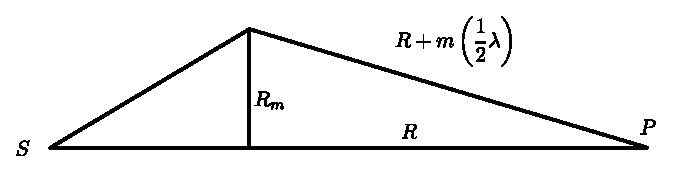
\includegraphics[height=1.7cm]{images/fresnel-radius.eps}
				% \vspace{1em}
			\end{center}
			Nach dem Satz des Pythagoras gilt:
			\begin{align}
				\left(R+\frac{m}{2}\lambda\right)^2 &= R_m^2 + R^2 \\
				R_m^2 &= \left(R+\frac{m}{2}\lambda\right)^2 - R^2 = \left[\cancel{R^2} + \frac{m^2}{2}\lambda^2 + \cancel{2}R\left(\frac{m}{\cancel{2}}\lambda\right)\right] - \cancel{R^2} \notag \\
				&= mR\lambda + \frac{m^2}{2}\lambda^2
			\end{align}
			In unserer Betrachtung ist $R \gg \lambda$, also gilt die Annährung:
			\begin{align}
				R_m^2 \approx mR\lambda &&\implies&& R_m = \sqrt{mR\lambda}
			\end{align}
			was zu zeigen ist. 

		\item \question{Welche Spaltbreite ergibt sich somit beim Aufspalten der Zentralmaximums des Fraunhoferschen Beugungsbildes in zwei Maxima, die durch ein minimum getrennt sind? Berechnen Sie diesen Wert. Ist er realistisch?}

			Beim Aufspalten der Zentralmaximums des Fraunhoferschen Beugungsbildes in zwei Maxima ist genau zwei Fresnel-Zone beteiligt. Die Spaltbreite muss somit $2\cdot R_2$ entsprechen. 

			In dem Versuch ist $R=\SI{30.0(5)}{\centi\meter}$. Da wir während des Versuchs keine Aufwäremzeit berücksichtigt haben, könnte die Wellenlänge des Laser ($\lambda = \SI{632.9}{\nano\meter}$) vom Erwartungswert schwanken. Wir wollen hier aber nur eine Abschätzung machen, deswegen sind alle Fehler vernachlässigt.

			Die benötigte Spaltbreite ist somit gegeben durch:
			\begin{align}
				b &= 2\cdot R_2 = 2\sqrt{2R\lambda} = 2\sqrt{2(\SI{0.300}{\meter})\left(\SI{632.9e-9}{\meter}\right)} \notag \\
				&= \SI{1.23e-3}{\meter} = \SI{1.23}{\milli\meter} \sigfig{3}
			\end{align}
			Diese Breite ist realistisch. 
	\end{itemize}
	

